\section{Resposta a um curto-circuito}
\begin{frame}
\frametitle{Diagrama unifilar}
\begin{figure}[h!]
\begin{center}
    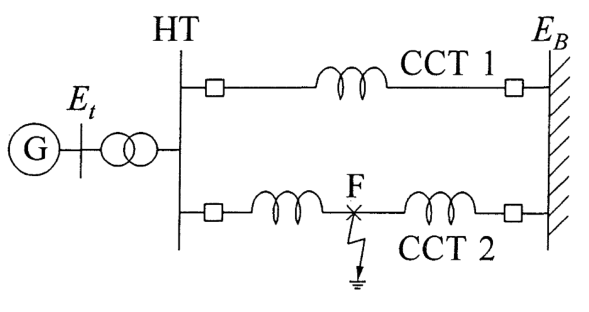
\includegraphics[width=10cm]{imagens/maq6.png}  
\end{center}
%\caption{Resultado prático da planta em malha aberta.}
\label{maq6} 
\end{figure}
\end{frame}

\begin{comment}
\begin{frame}
\frametitle{Circuito equivalente}
\begin{figure}[h!]
\begin{center}
    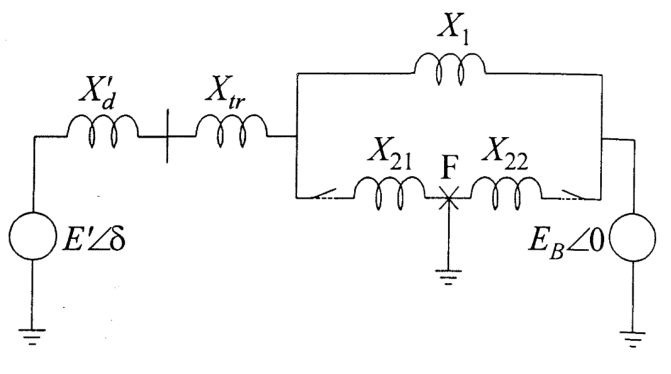
\includegraphics[width=10cm]{imagens/maq7.png}  
\end{center}
%\caption{Resultado prático da planta em malha aberta.}
\label{maq7} 
\end{figure}
\end{frame}
\end{comment}


\begin{frame}
\frametitle{Resposta para faltas - caso estável e instável}
\begin{figure}[h!]
\begin{center}
    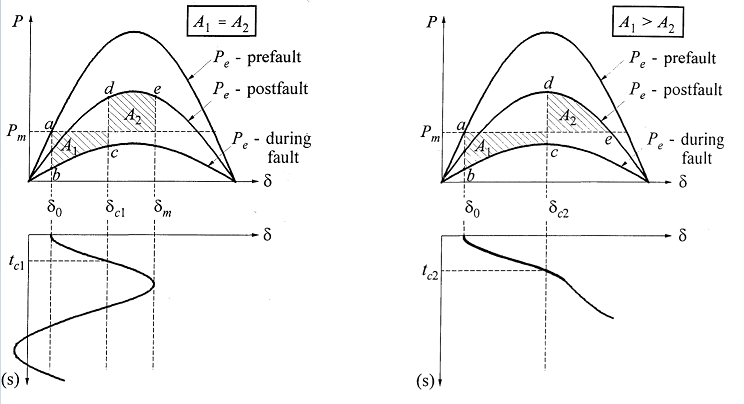
\includegraphics[width=12cm]{imagens/maq10.png}  
\end{center}
%\caption{Resultado prático da planta em malha aberta.}
\label{maq10} 
\end{figure}
\end{frame}




